\section{Simulation}

%\subsection{Expected physics performance}

%A series MC simulation have been used to calculate the acceptance of the central detector and have reconstructed physics parameters for types of events that are of interest. Fig. ... shows the missing mass resolution expected for MC simulation studies for a number of different reactions. For all cases studied, the results show that it is possible to identify the missing particle for each reaction.
%Figure ... shows the missing mass spectrum expected when pion is detected in the central tracker. There is sufficient resolution to study resonant production and to compare, for example, s, t, and u channel processes.

\subsection{Detector simulation}

A realistic model of the SVT has been developed, describing the location and composition of all modules, with material description based on the engineering drawings and assembly procedures, and confirmed by the survey measurements during integration. The SVT design and module layout were validated by Geant-4-based simulated detector performance studies demonstrating compliance with the technical requirements and engineering models. A 3D view of the simulated geometry of the SVT sensors is shown in Fig.~\ref{fig:svt3dview}. The SVT model is described in the simulation article of this volume. 

\begin{figure}[hbt] 
\centering 
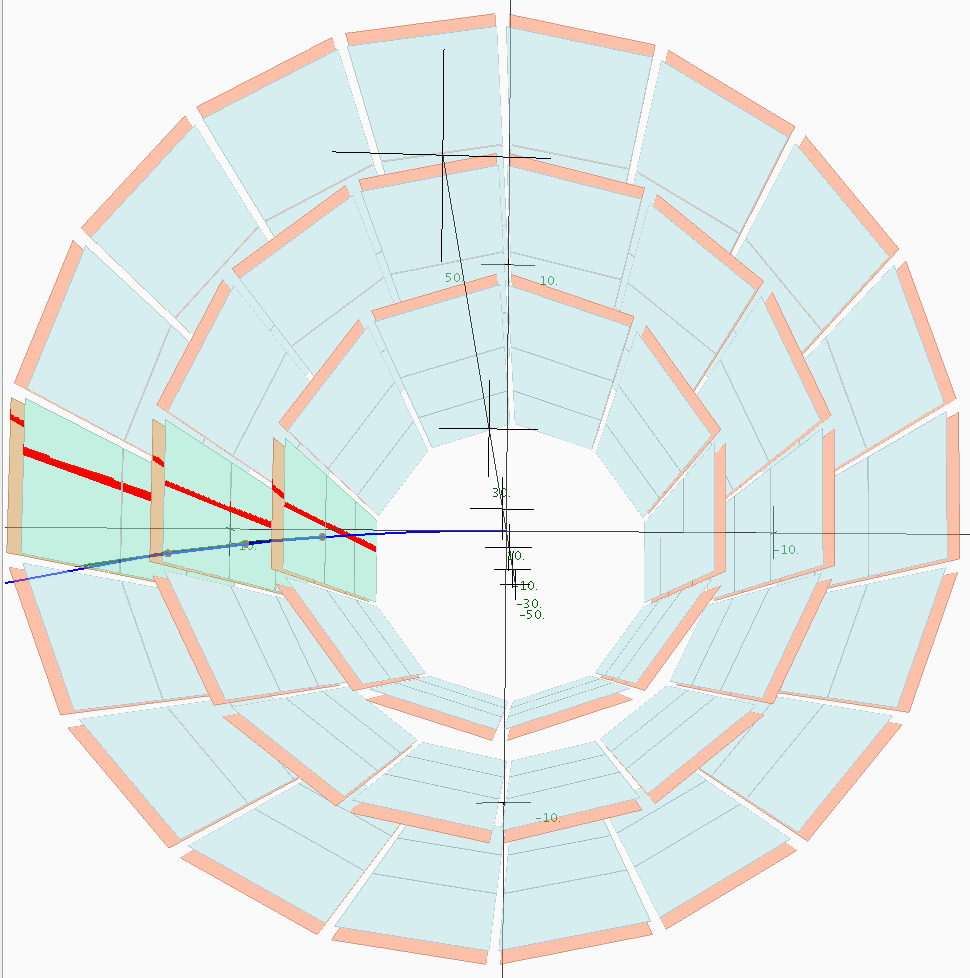
\includegraphics[width=1.0\columnwidth,keepaspectratio]{svt3dview.png}
\caption{3D view of the simulated SVT detector geometry.}
\label{fig:svt3dview}
\end{figure}

According to the results of GEANT simulation of the SVT, a resolution of 50~$\mu$m in the bending plane is needed to measure, with a precision better than 5$\%$, tracks with momentum up to 1~GeV (see Fig.~\ref{fig:PtRes}) \cite{MC1,MC2}. At low momenta the degradation of the resolution is caused by multiple scattering.

\begin{figure}[hbt]
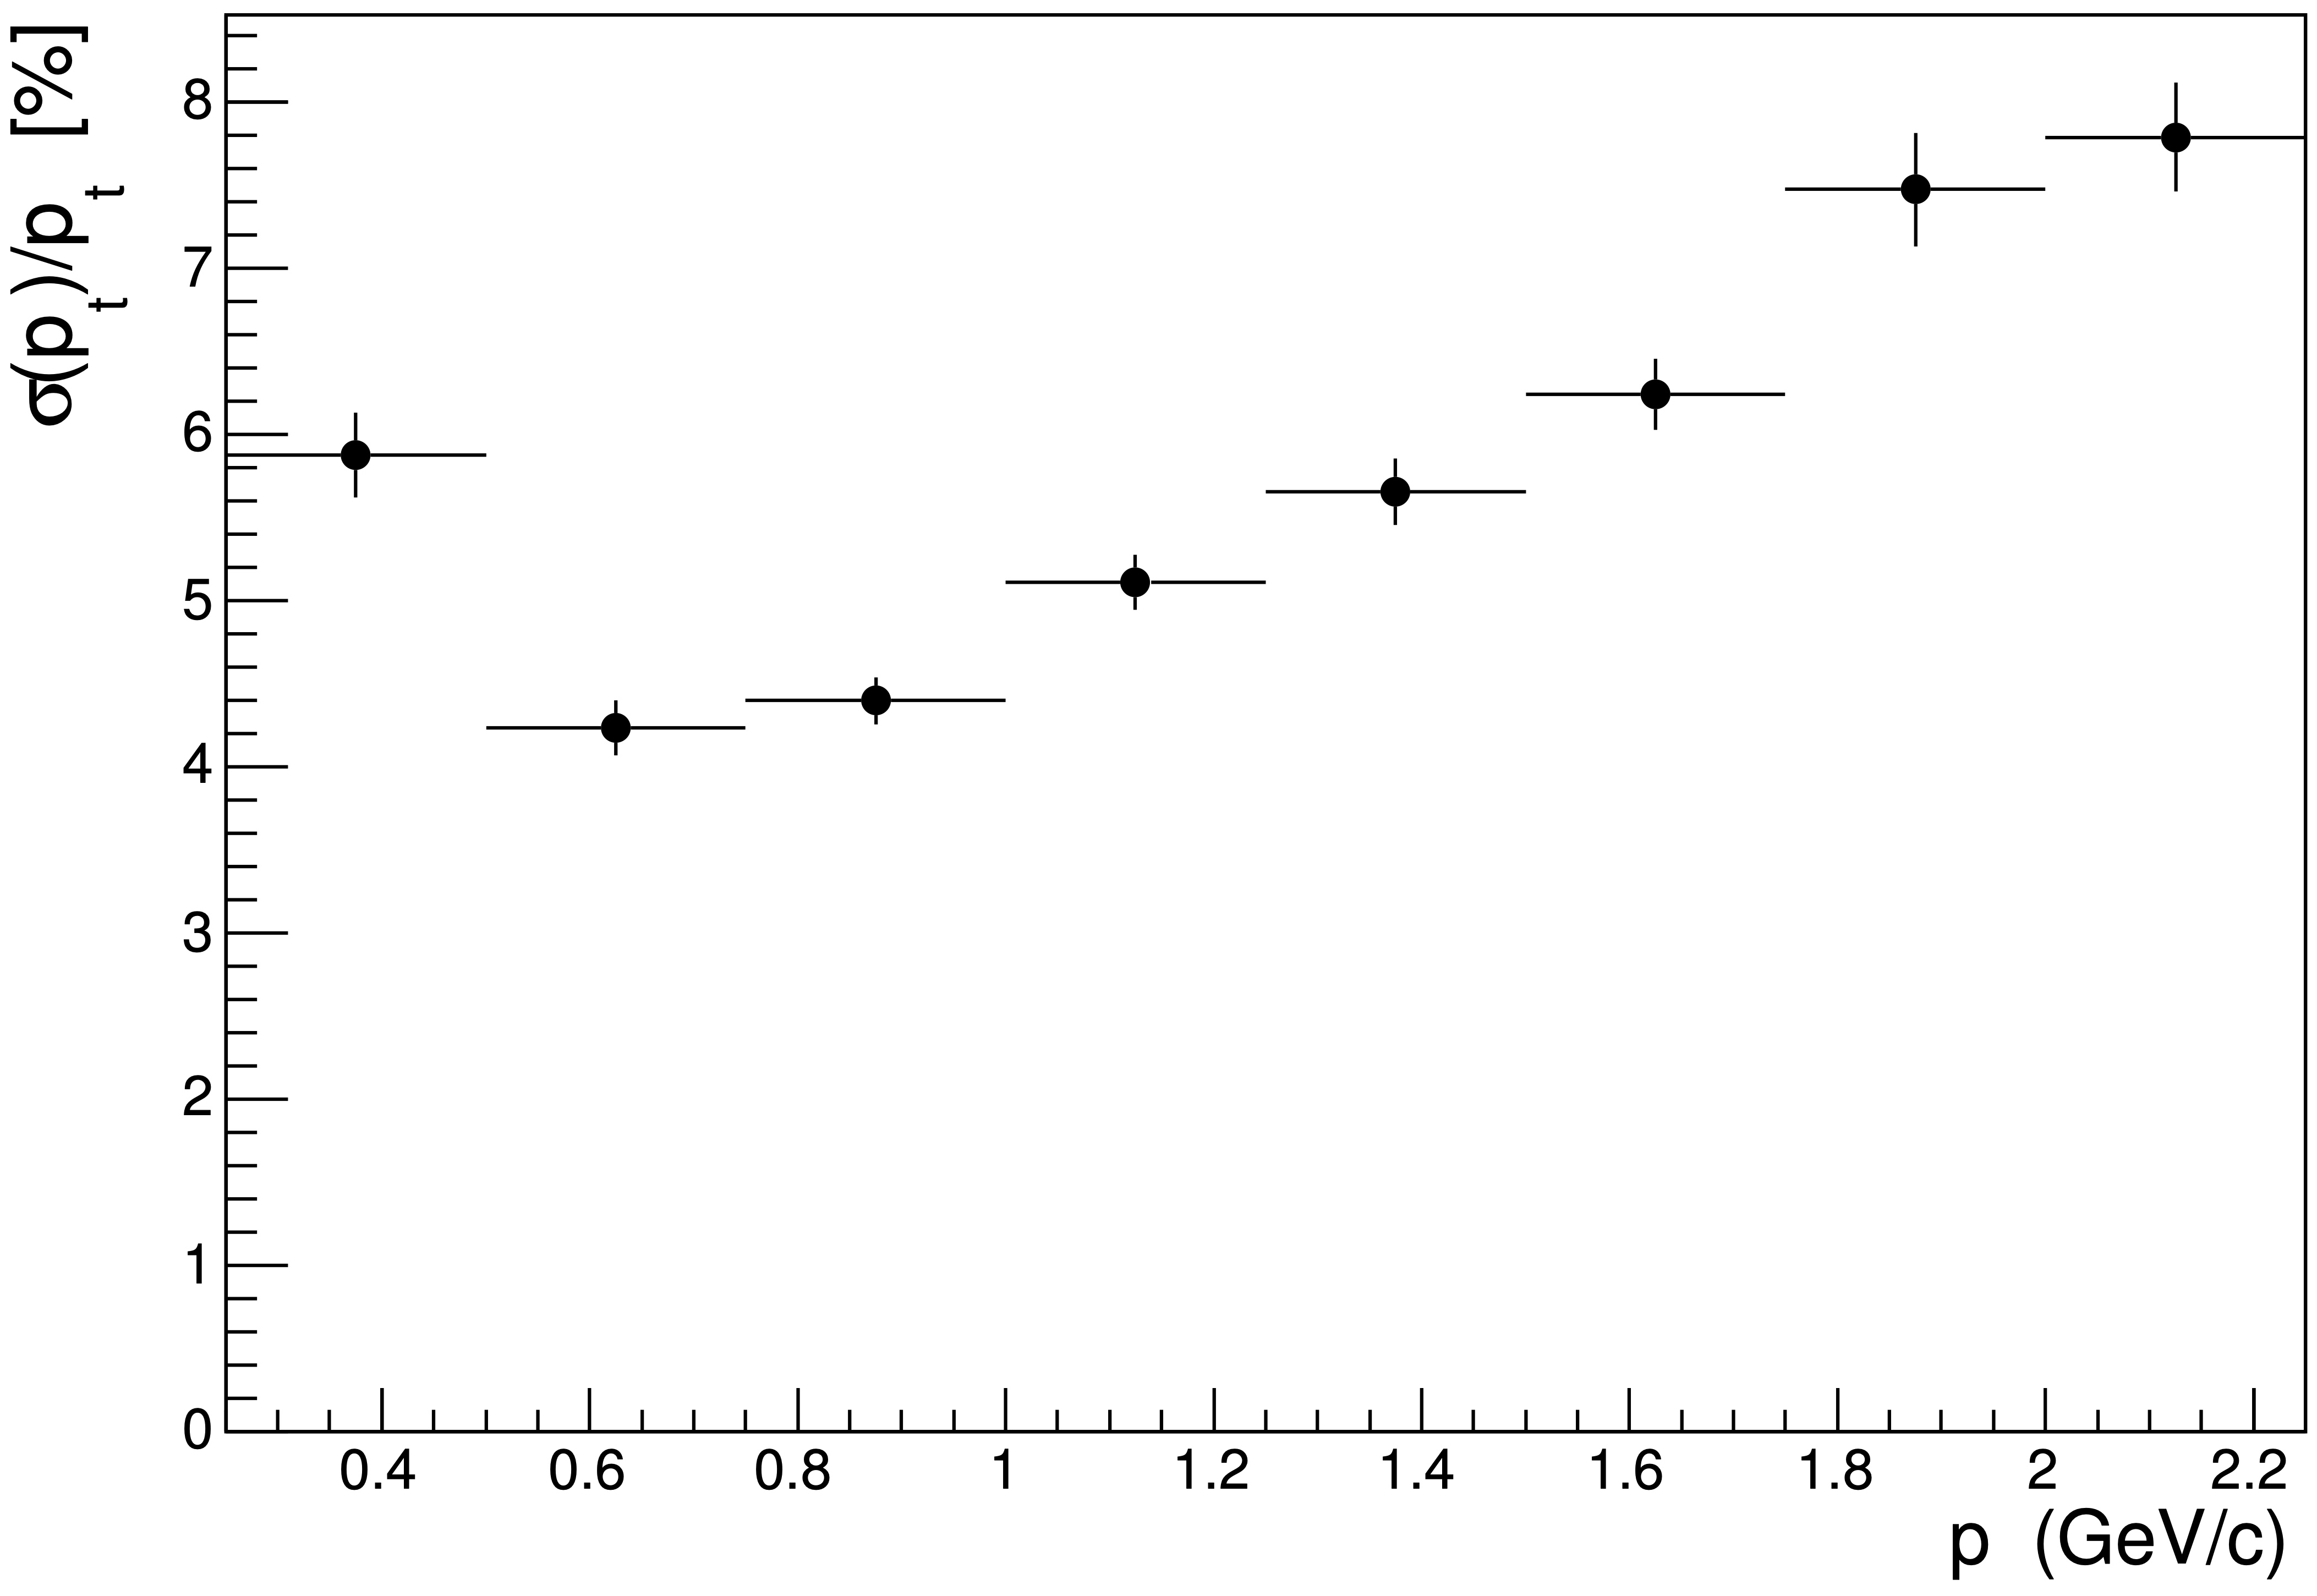
\includegraphics[width=1.0\columnwidth,keepaspectratio]{PtResol.jpg}
\caption{Simulated SVT momentum resolution.}
\label{fig:PtRes}
\end{figure}

Centroid residual distribution for the simulated muon tracks generated in the interval 0.5--2 GeV is shown in Fig.~\ref{fig:centroid-residual-mc}. Cluster centroids were calculated based on the charge weighting method. The spacial resolution of the sensors in the transverse plane using the ideal SVT geometry with no misalignments was found to be about 30~$\mu$m. 

\begin{figure}[hbt]
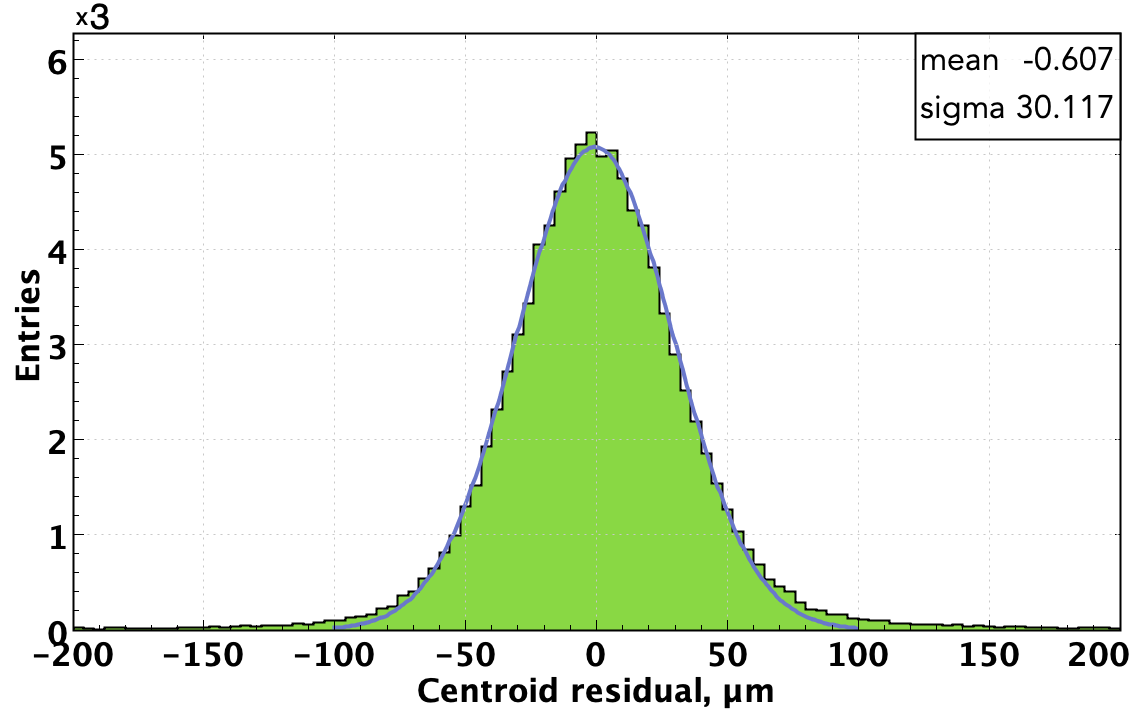
\includegraphics[width=1.0\columnwidth,keepaspectratio]{centroid-residual-mc.png}
\caption{Simulated centroid residual distribution for the SVT module.}
\label{fig:centroid-residual-mc}
\end{figure}

\subsection{Backgrounds, energy deposition, dose rates}

Radiation-induced bulk and surface detector damage studies have been conducted with charged hadrons, leptons, neutrons, and $\gamma$-ray photons. The radiation damage produced by different particles with different energies are scaled under the assumption of the Non-Ionizing Energy Loss (NIEL) hypothesis as the radiation damage in the silicon bulk depends only on the non-ionizing energy loss. The damage caused by different particles is referenced to the damage from 1 MeV neutrons. The standard value for the NIEL of 1 MeV neutrons is 95 MeVmb. 

\begin{figure}[hbt] 
\centering 
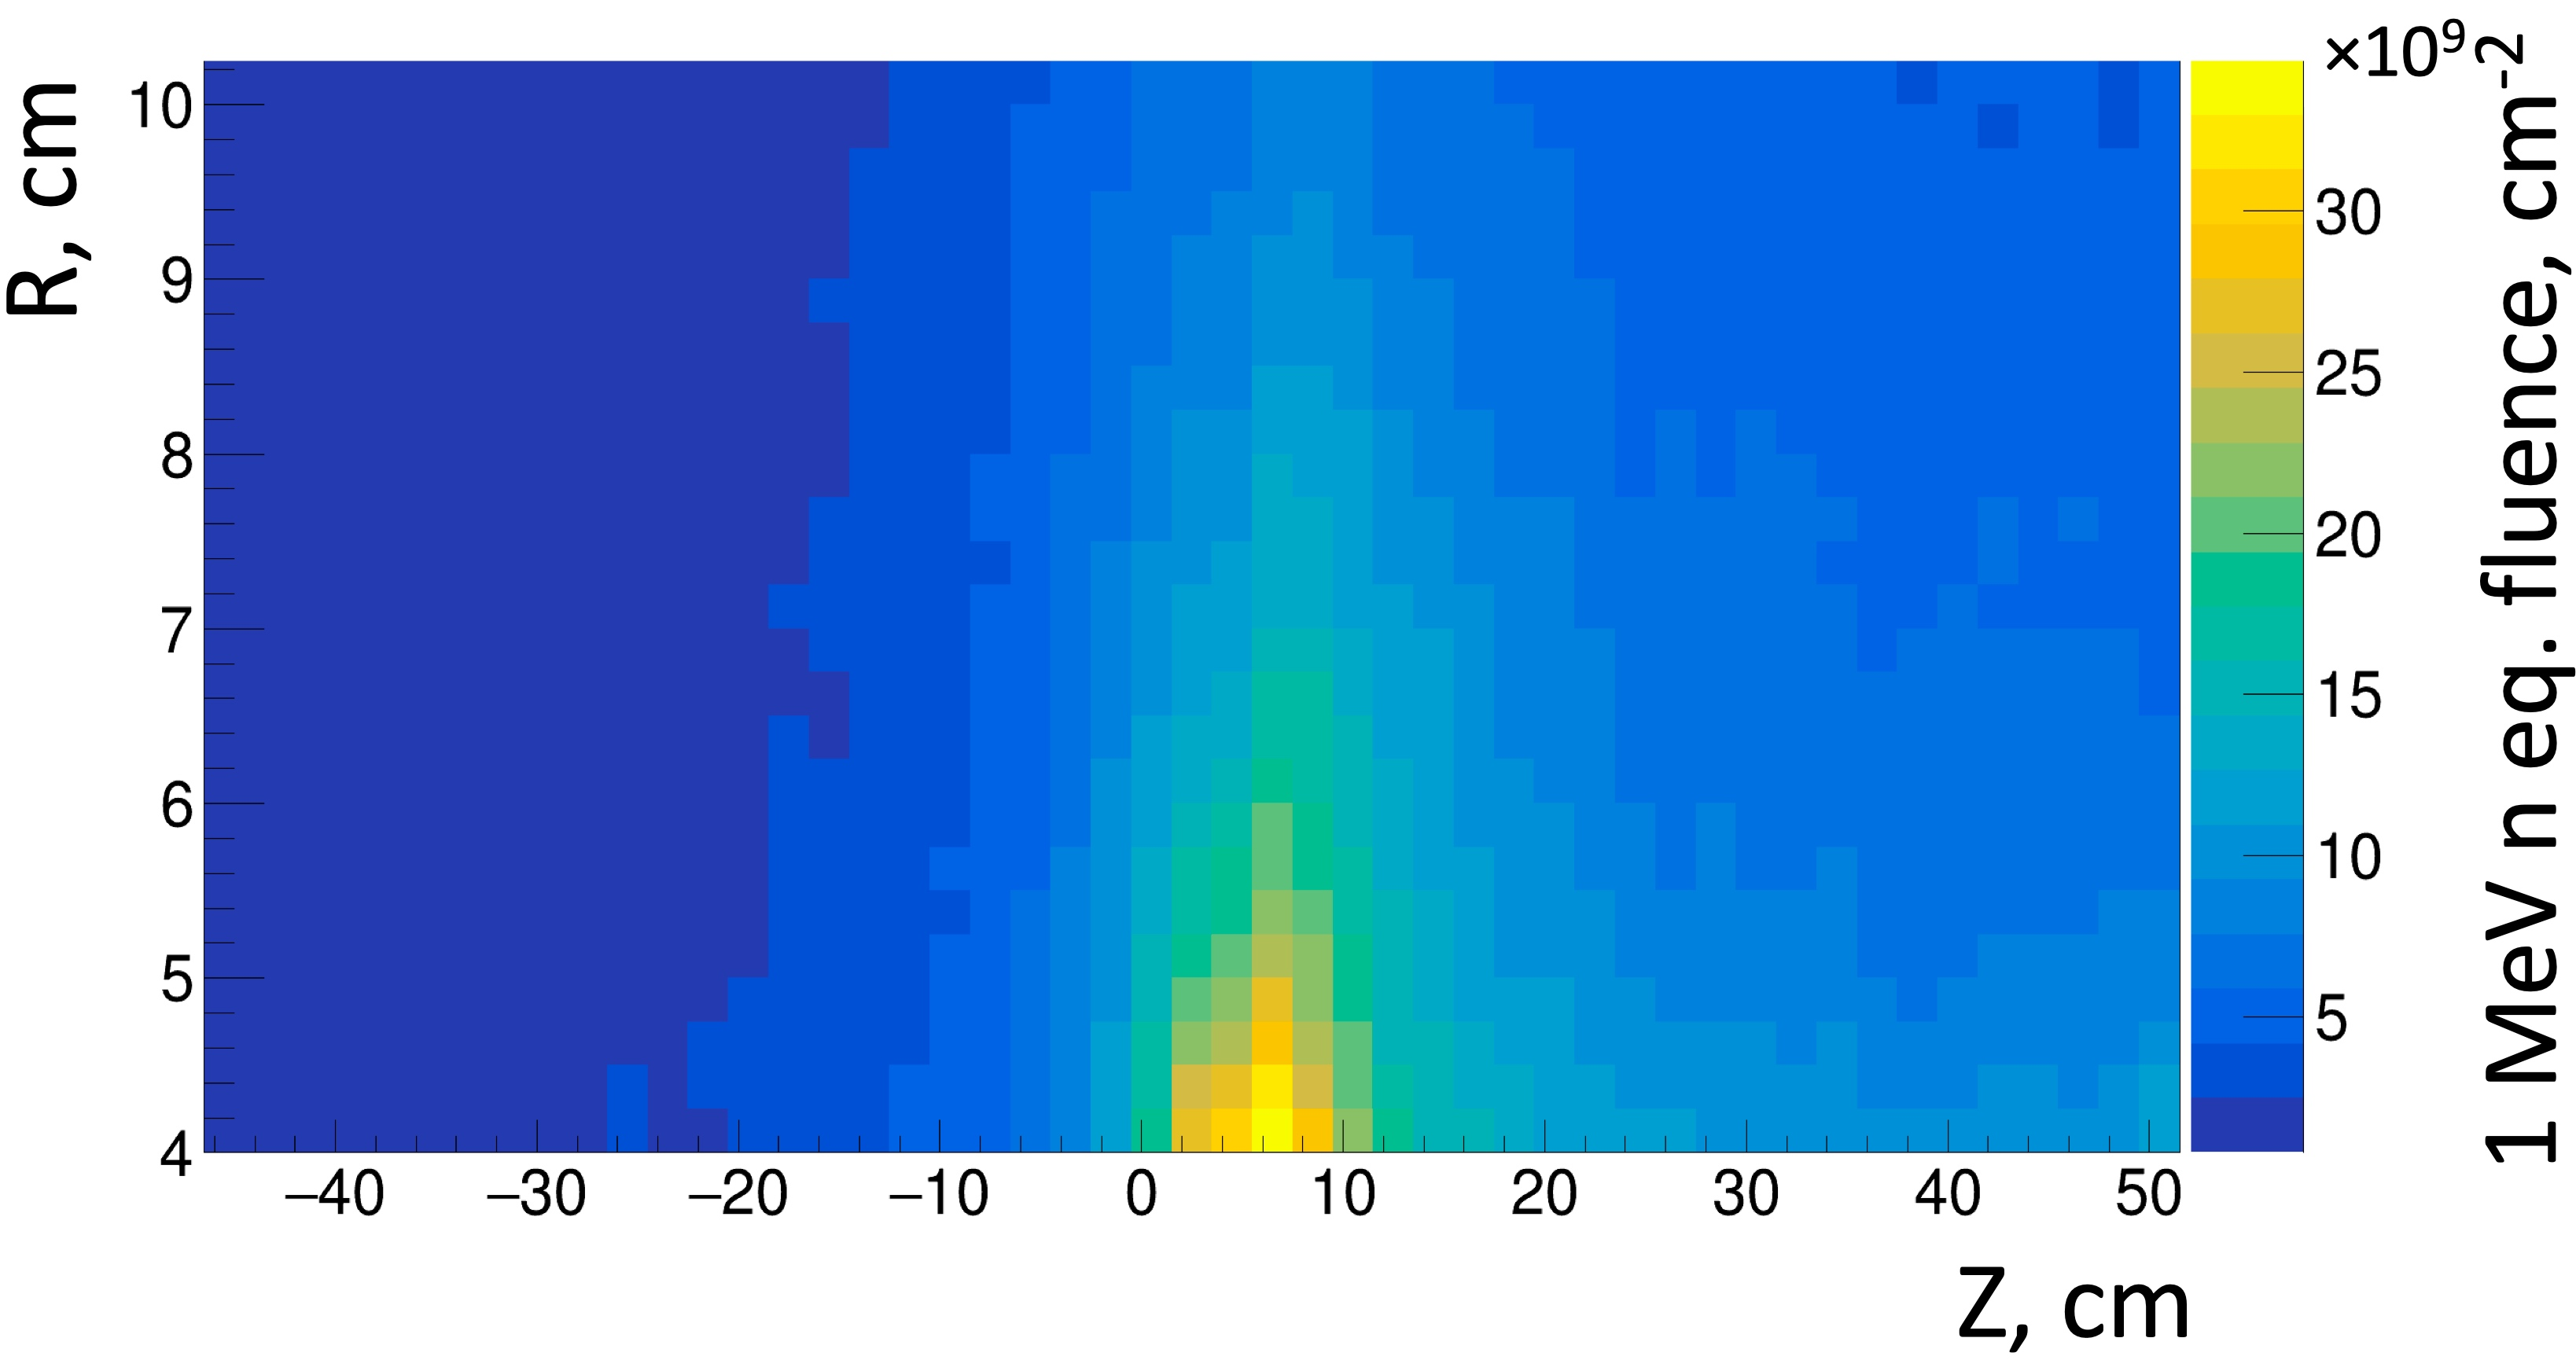
\includegraphics[width=1.0\columnwidth,keepaspectratio]{Pb_1MeVeq.jpg}
\caption{Accumulated 1MeV equivalent neutron fluence for the lead target.}
\label{fig:fluka1}
\end{figure}

To calculate the effects of different target configurations on the SVT detector,  FLUKA~\cite{FLUKA1, FLUKA2} simulations have been performed. In order to include the hadron electro-nuclear production, a dedicated source term has been used to enhance the physics production from the target, since it is a key in radiation estimates for targets with radiation length below 4$\%$. To assess the radiation damage to the SVT, the accumulated 1MeV neutron equivalent fluence has been recorded corresponding to the planned run conditions. For the experiment with lead target, the expected exposure was 240 h at beam current of 38 nA with electron beam energy of 6.6 GeV (Fig.~\ref{fig:fluka1}). For deuterium target, the study has been done for the accumulated charge of 108 mC at 11 GeV (Fig.~\ref{fig:fluka2}). In both scenarios the expected doses should not cause substantial degradation of the silicon sensors.

\begin{figure}[hbt] 
\centering 
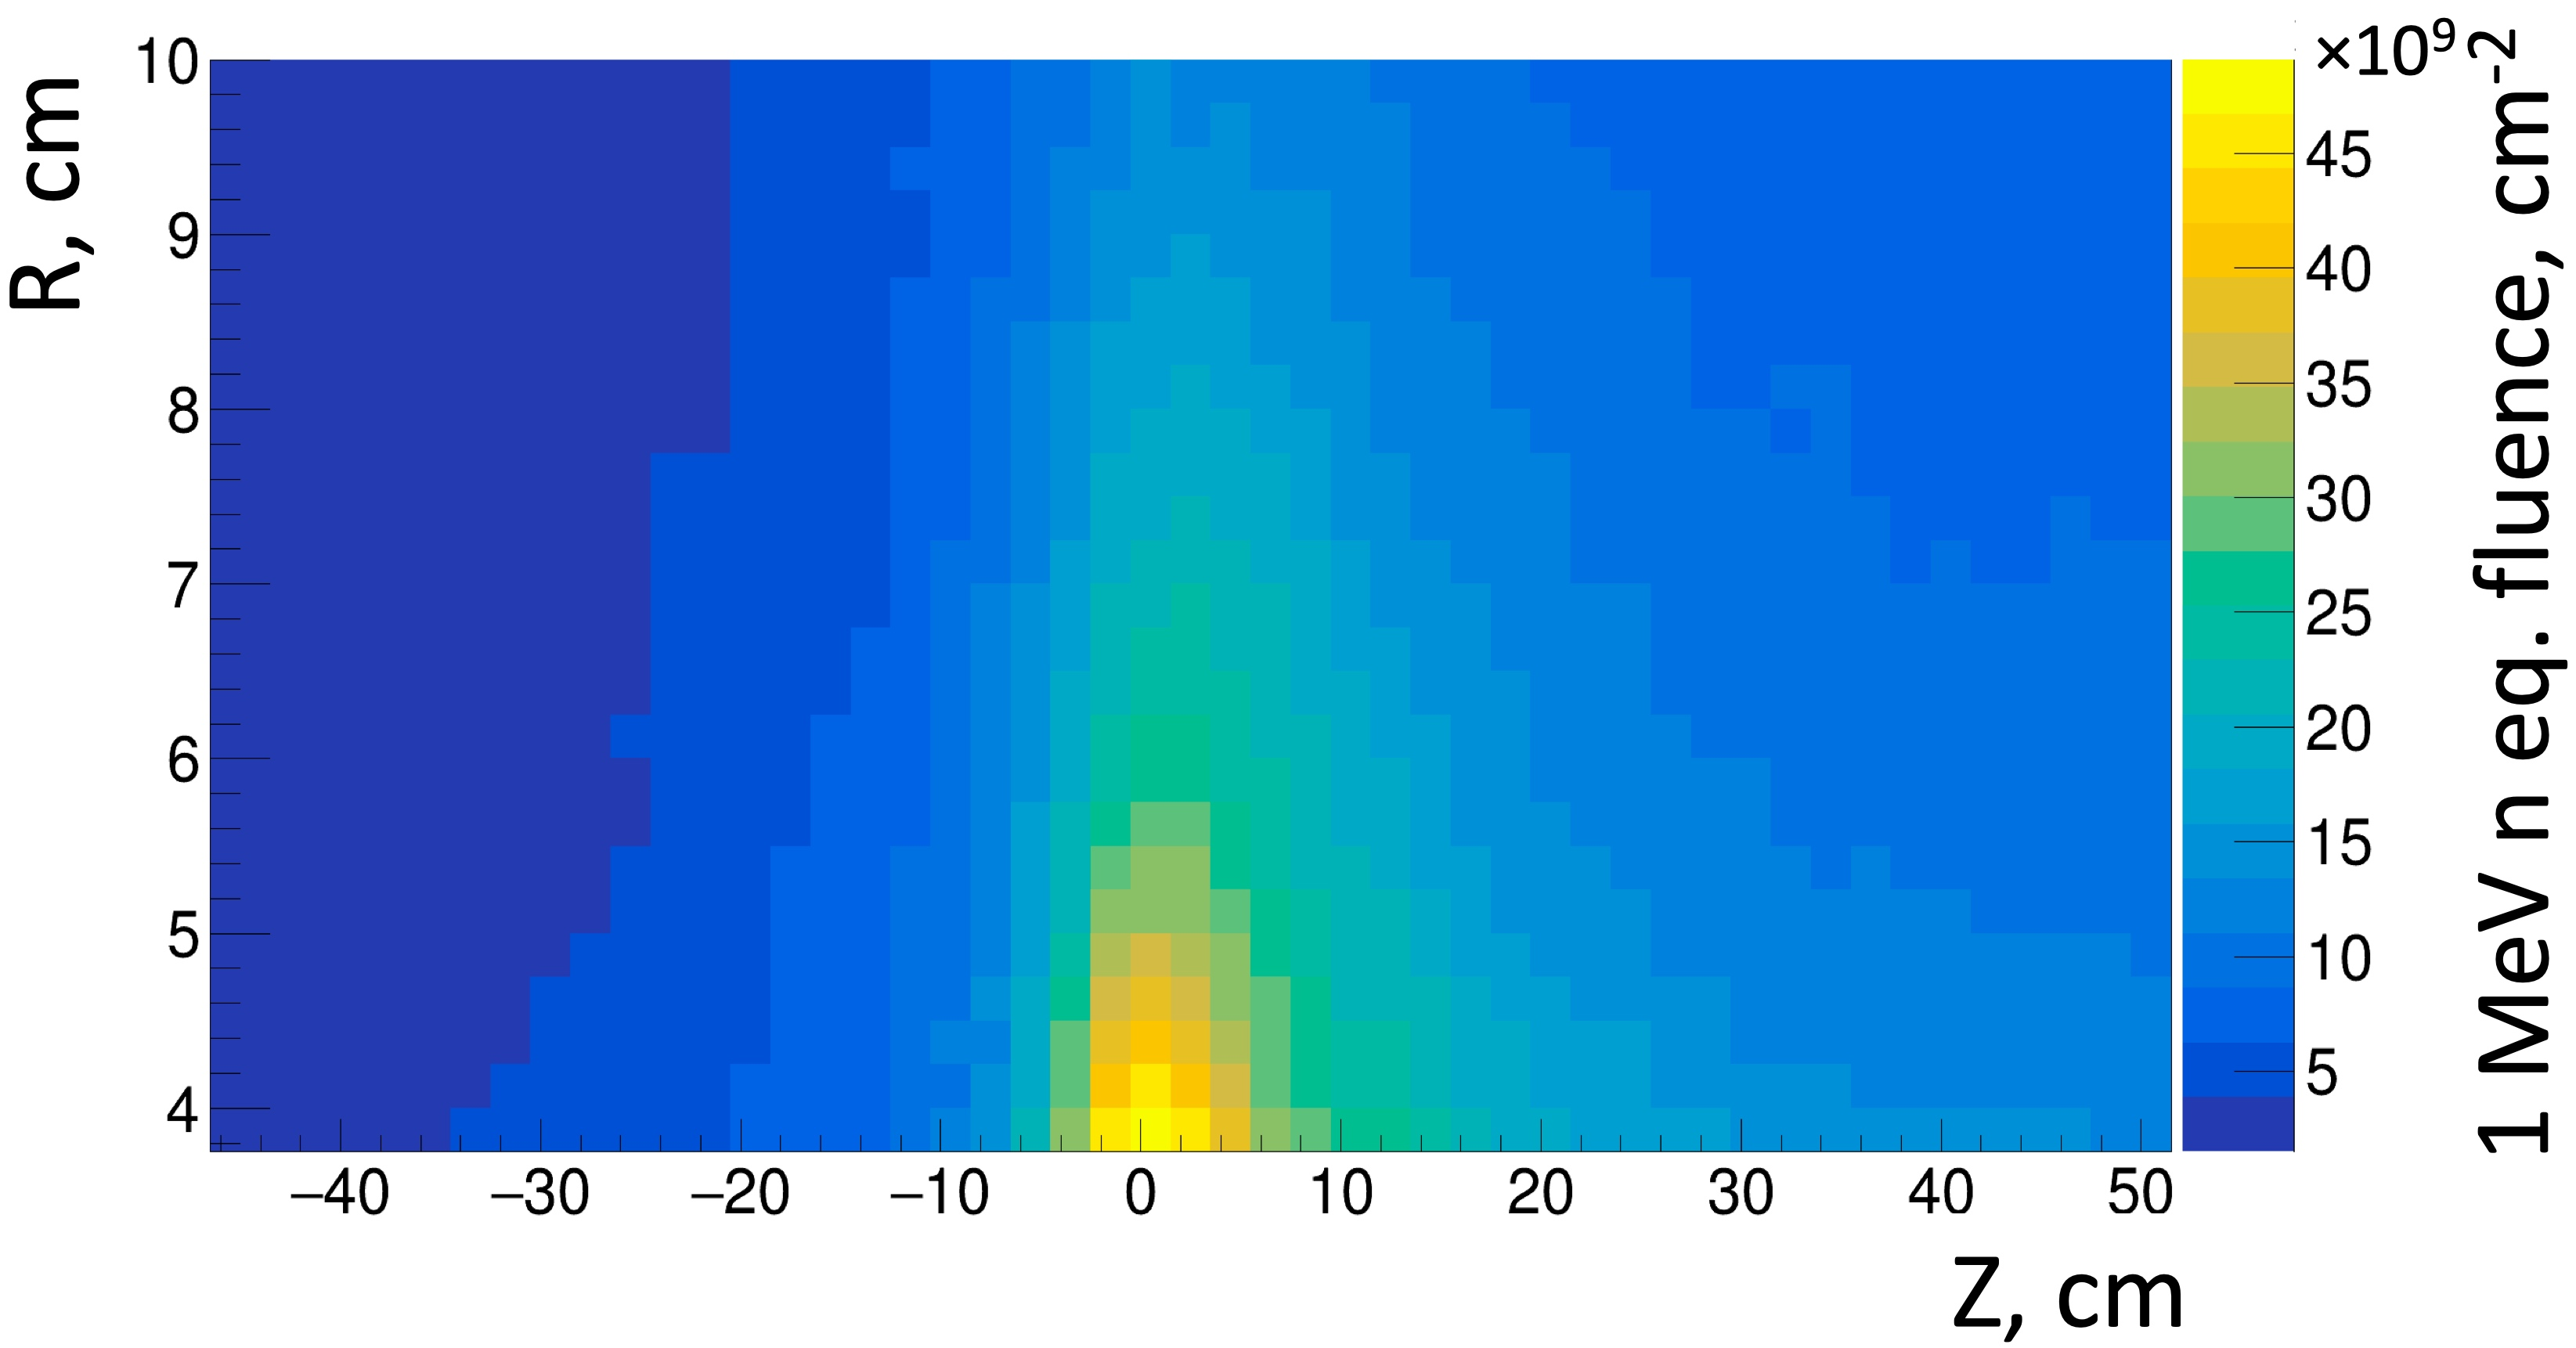
\includegraphics[width=1.0\columnwidth,keepaspectratio]{Deuterium_1MeVeq.jpg}
\caption{Accumulated 1MeV equivalent neutron fluence for the deuterium target.}
\label{fig:fluka2}
\end{figure}

FLUKA simulations of radiation damage levels have been performed in terms of 1MeV equivalent neutron fluence and high energy hadron equivalent fluence which is proportional to the rate of Single Event Effects (SEE)~\cite{FLUKA3}. Estimated levels of radiation damage in radial direction are presented in Fig.~\ref{fig:rad-levels-radial}) for liquid hydrogen and carbon targets at nominal beam currents. Also shown the radiation levels for the tagger magnet yoke during the beam tuning (see the beam line section in this volume).

\begin{figure}[hbt] 
\centering 
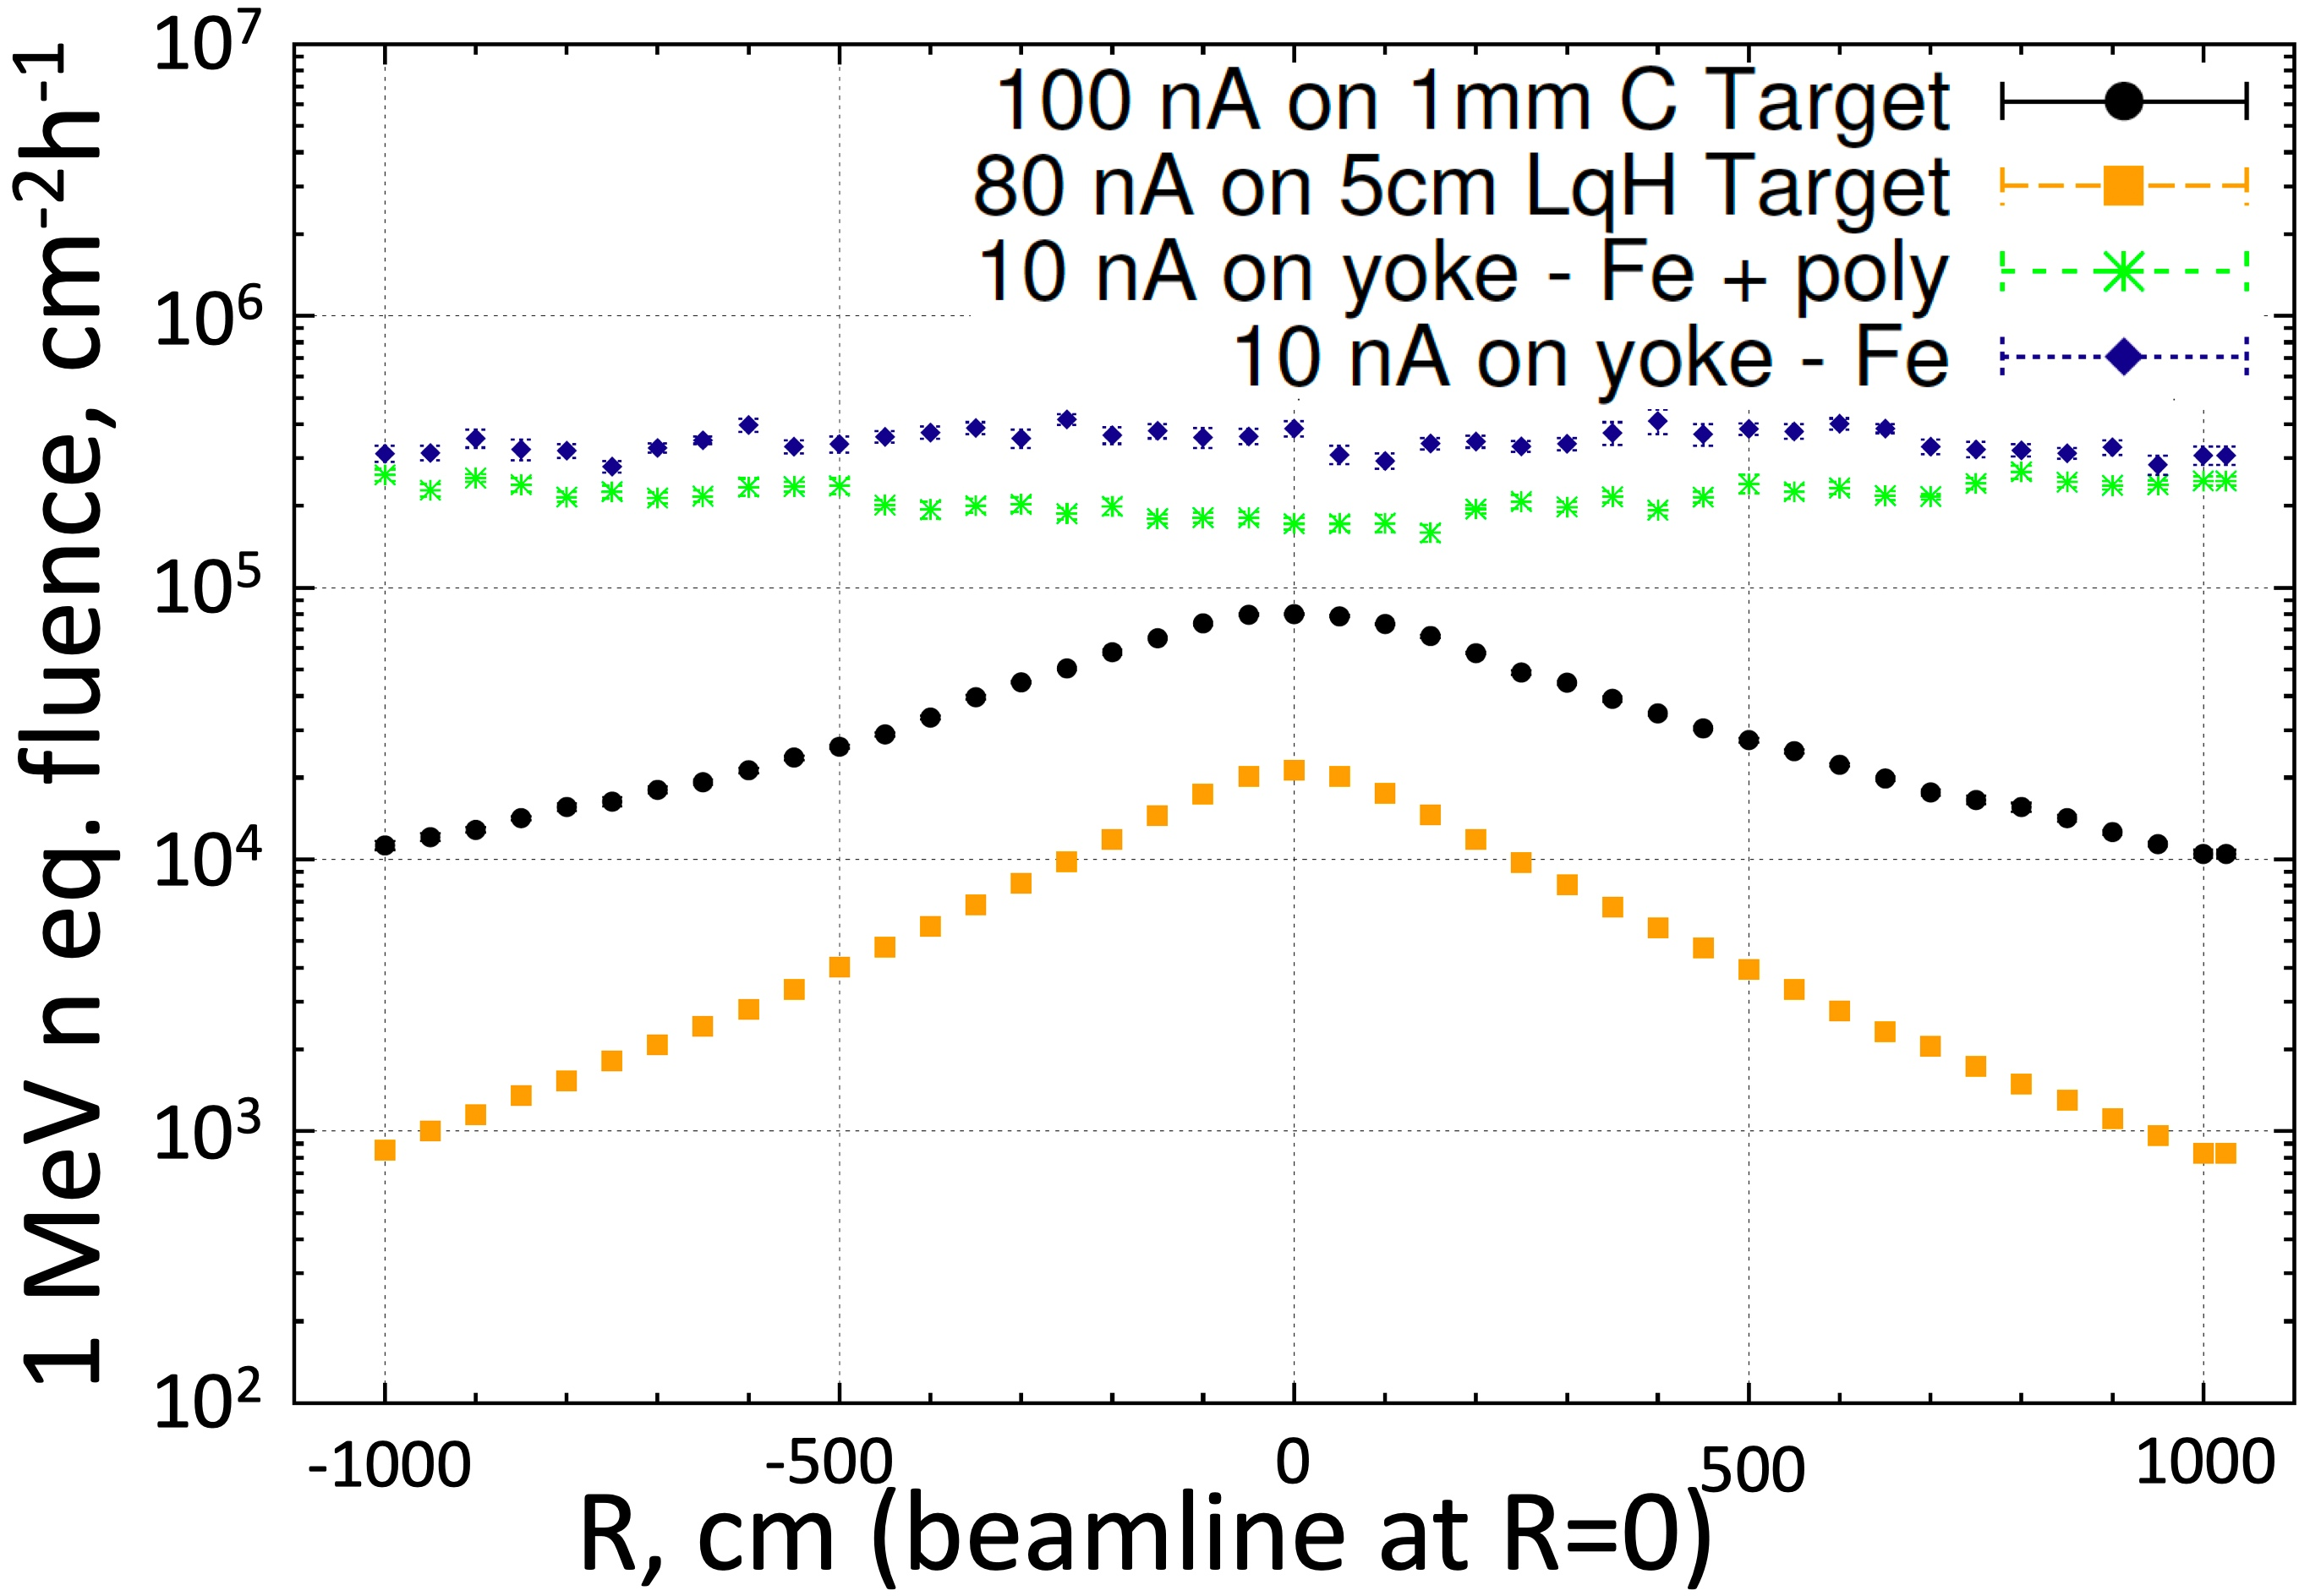
\includegraphics[width=1.0\columnwidth,keepaspectratio]{rad-levels-radial.jpg}
\caption{Estimated levels of radiation damage in radial direction in terms of 1MeV neutron equivalent fluence in silicon.}
\label{fig:rad-levels-radial}
\end{figure}

Simulations of beam-related backgrounds were performed for several thicknesses of a tungsten shielding cylinder around the CLAS12 target covering the first SVT layer. 
 
\begin{figure}[hbt] 
\centering 
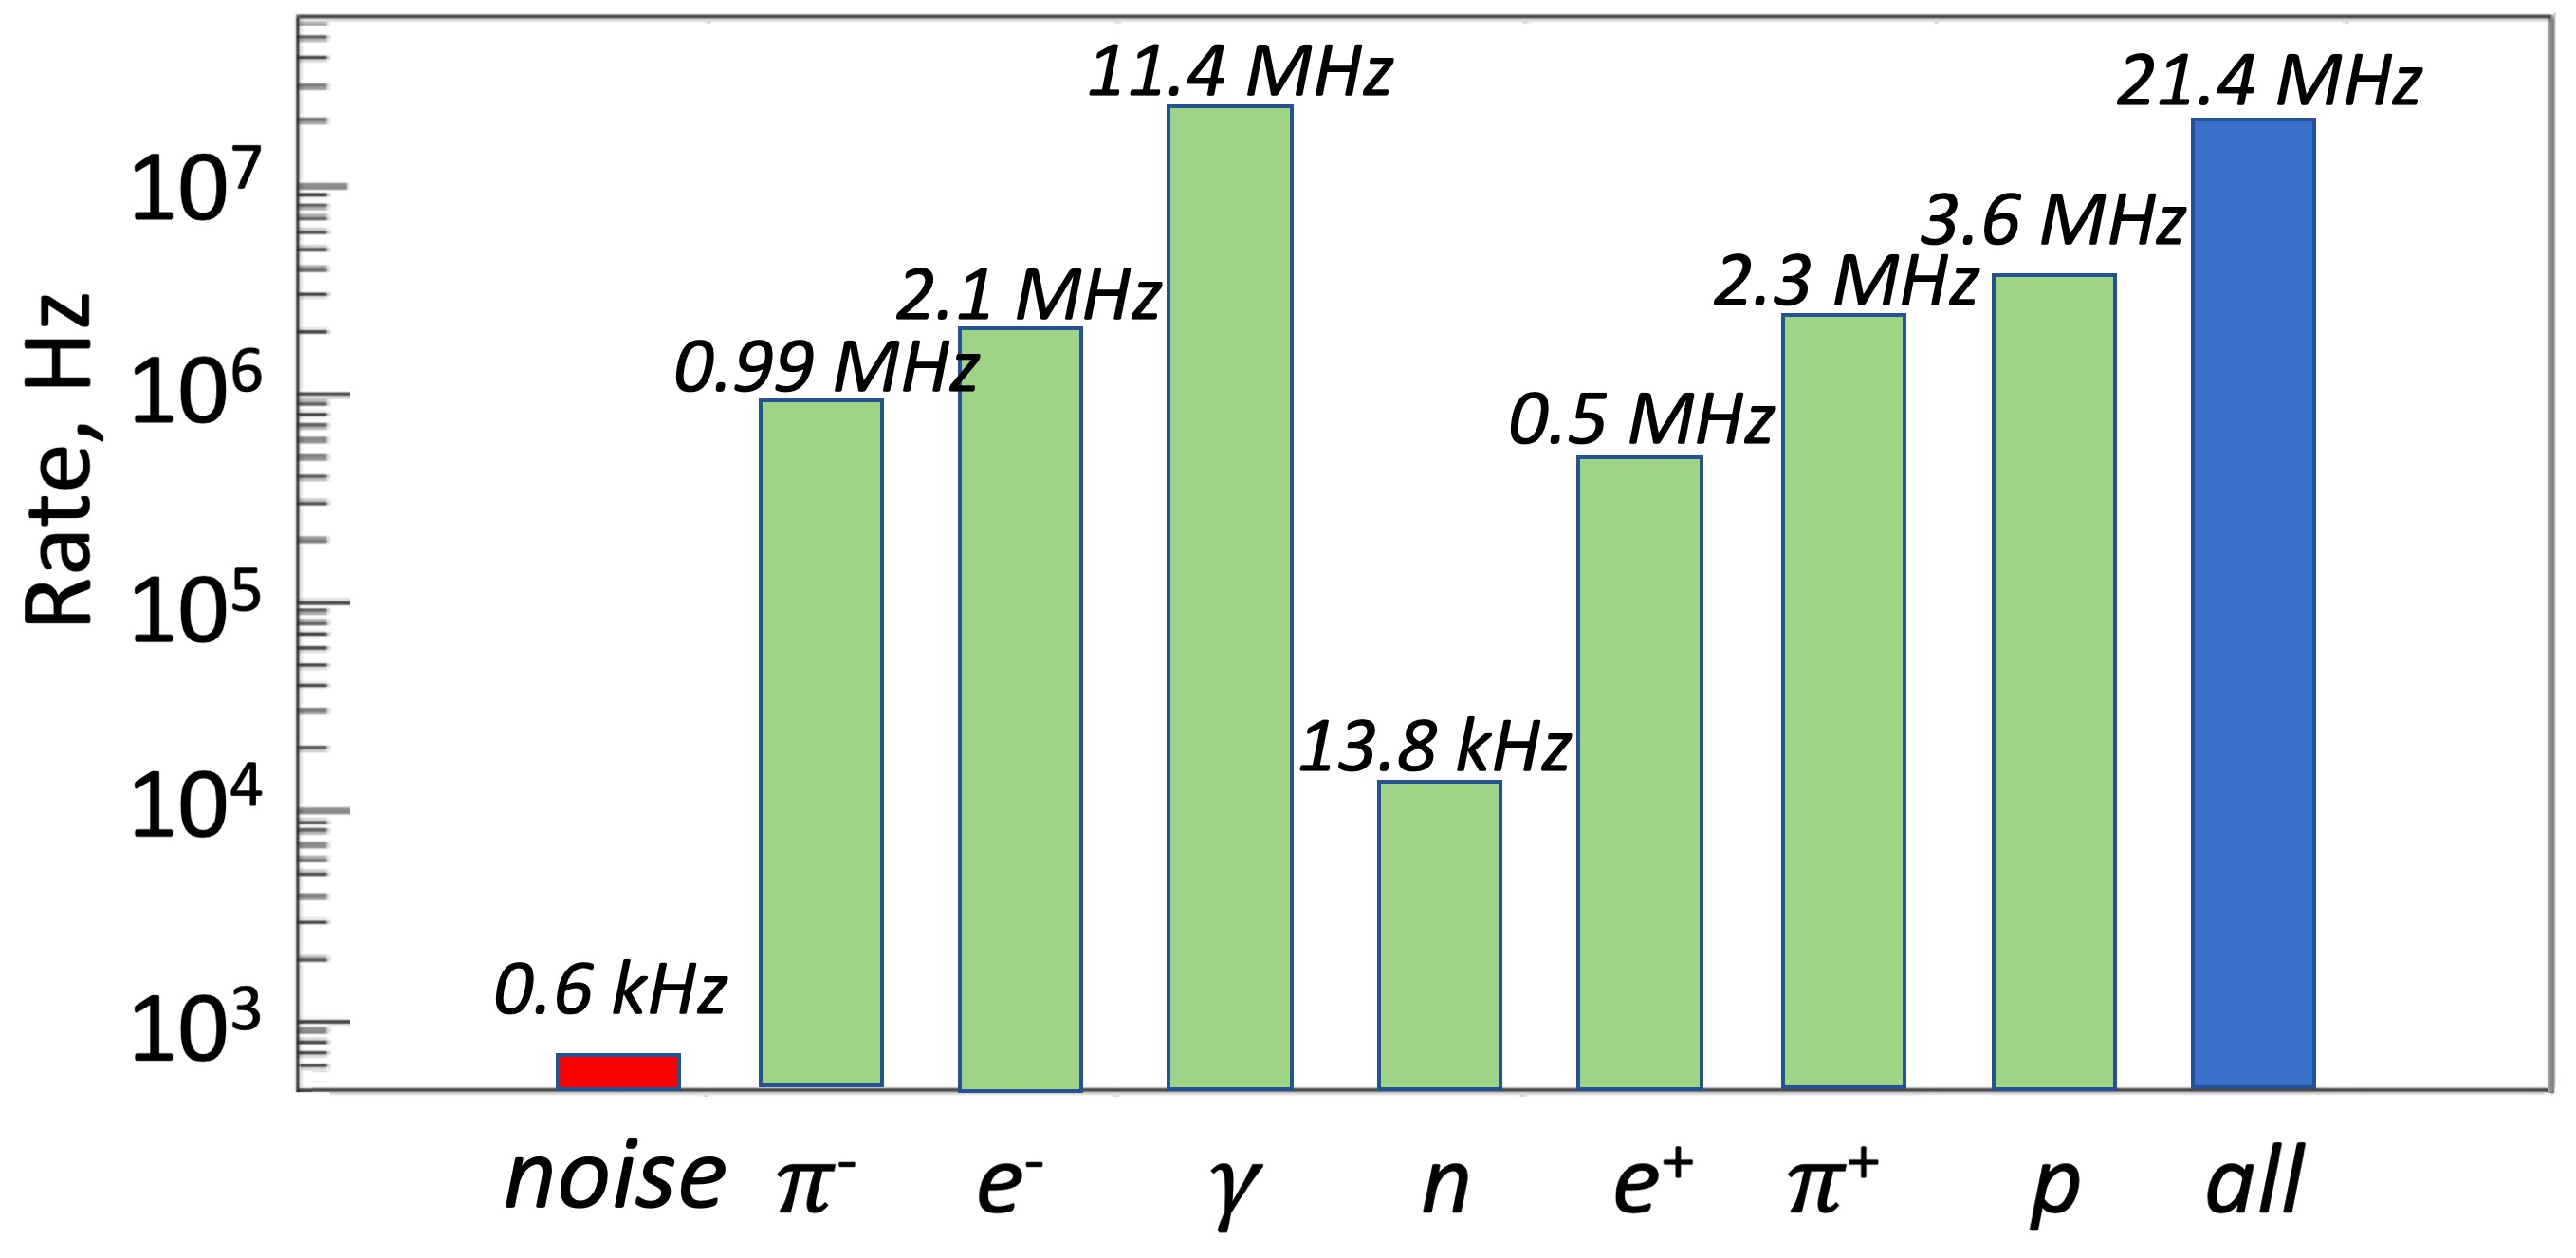
\includegraphics[width=1.0\columnwidth,keepaspectratio]{rates-lh2.jpg}
\caption{Rates in the first SVT layer for a 5-cm long liquid hydrogen target at the nominal CLAS12 operating luminosity of 10$^{35}$cm$^{-2}$s$^{-1}$.}
\label{fig:rates-lh2}
\end{figure}

Fluences, radiation doses, and 1 MeV neutron damage rates in the SVT were calculated for different particles. Rates were estimated for liquid hydrogen, liquid deuterium, carbon, iron, and lead targets. For each event, 124,000 electrons going through the target within a 248.5-ns time window were simulated. This corresponds to the full CLAS12' 10$^{35}$cm$^{-2}$s$^{-1}$ luminosity on a 5-cm-long liquid-hydrogen target at 11 GeV beam energy. Rates in the first SVT layer for a liquid-hydrogen target are shown in Fig.~\ref{fig:rates-lh2}. For carbon target at a threshold of 40 keV the hadronic rate was estimated to be 5 MHz (total rate 40 MHz) with strip hit rates of 3.1 kHz (region 1), 2.2 kHz (region 2), and 1.7 kHz (region 3). The energy deposited in layer 1 for the electromagnetic and the hadronic particles is shown in Fig.~\ref{fig:energy-deposited-l1}. At a threshold of 30 keV, 92$\%$ of the electromagnetic background is rejected while preserving  99.5$\%$ of the signals coming from the hadrons~\cite{TDRSVT}.

\begin{figure}[hbt] 
\centering 
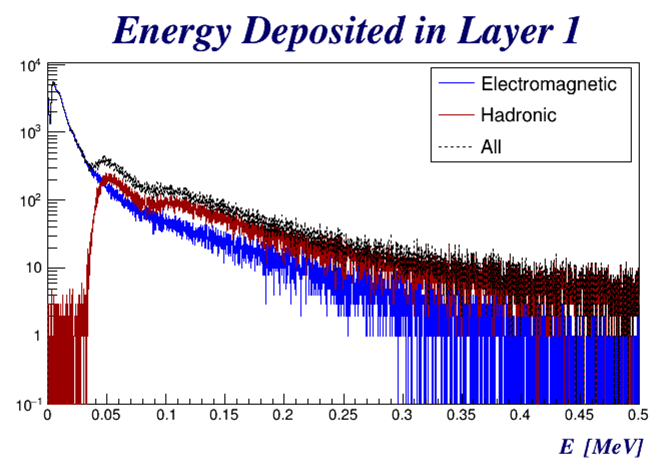
\includegraphics[width=1.0\columnwidth,keepaspectratio]{energy-deposited-l1.png}
\caption{Energy deposited in the SVT layer 1 for electromagnetic and hadronic particles for a liquid hydrogen target at the nominal CLAS12 operating luminosity.}
\label{fig:energy-deposited-l1}
\end{figure}

A tungsten shield 51~$\mu$m thick is installed on the target scattering chamber. The shield consists of 2 sheets mounted over the top and bottom halves of the foam cylinder referenced to the SVT common ground. The SVT rates and radiation damage benefit from the inclusion of the tungsten shield. The rates have been compared with physics run data at several beam currents. There is a good agreement between the real and the simulated data.

While the gamma fluences / doses show a dramatic decrease with the introduction of shielding, the total fluences and doses decrease significantly for the thinner configuration and do not vary much for thicker tungsten (see Fig.~\ref{fig:rates-l1}). The photon radiation dose becomes negligible for 50 $\mu$m or more of tungsten with total 1 MeV equivalent radiation dose about 65 krad per year on a liquid-hydrogen target. For 15 years of running the experiment on a carbon target the estimated radiation dose for the sensors is 2.5~Mrad (with 50 $\%$ operation) \cite{TDRSVT}. 

\begin{figure}[hbt] 
\centering 
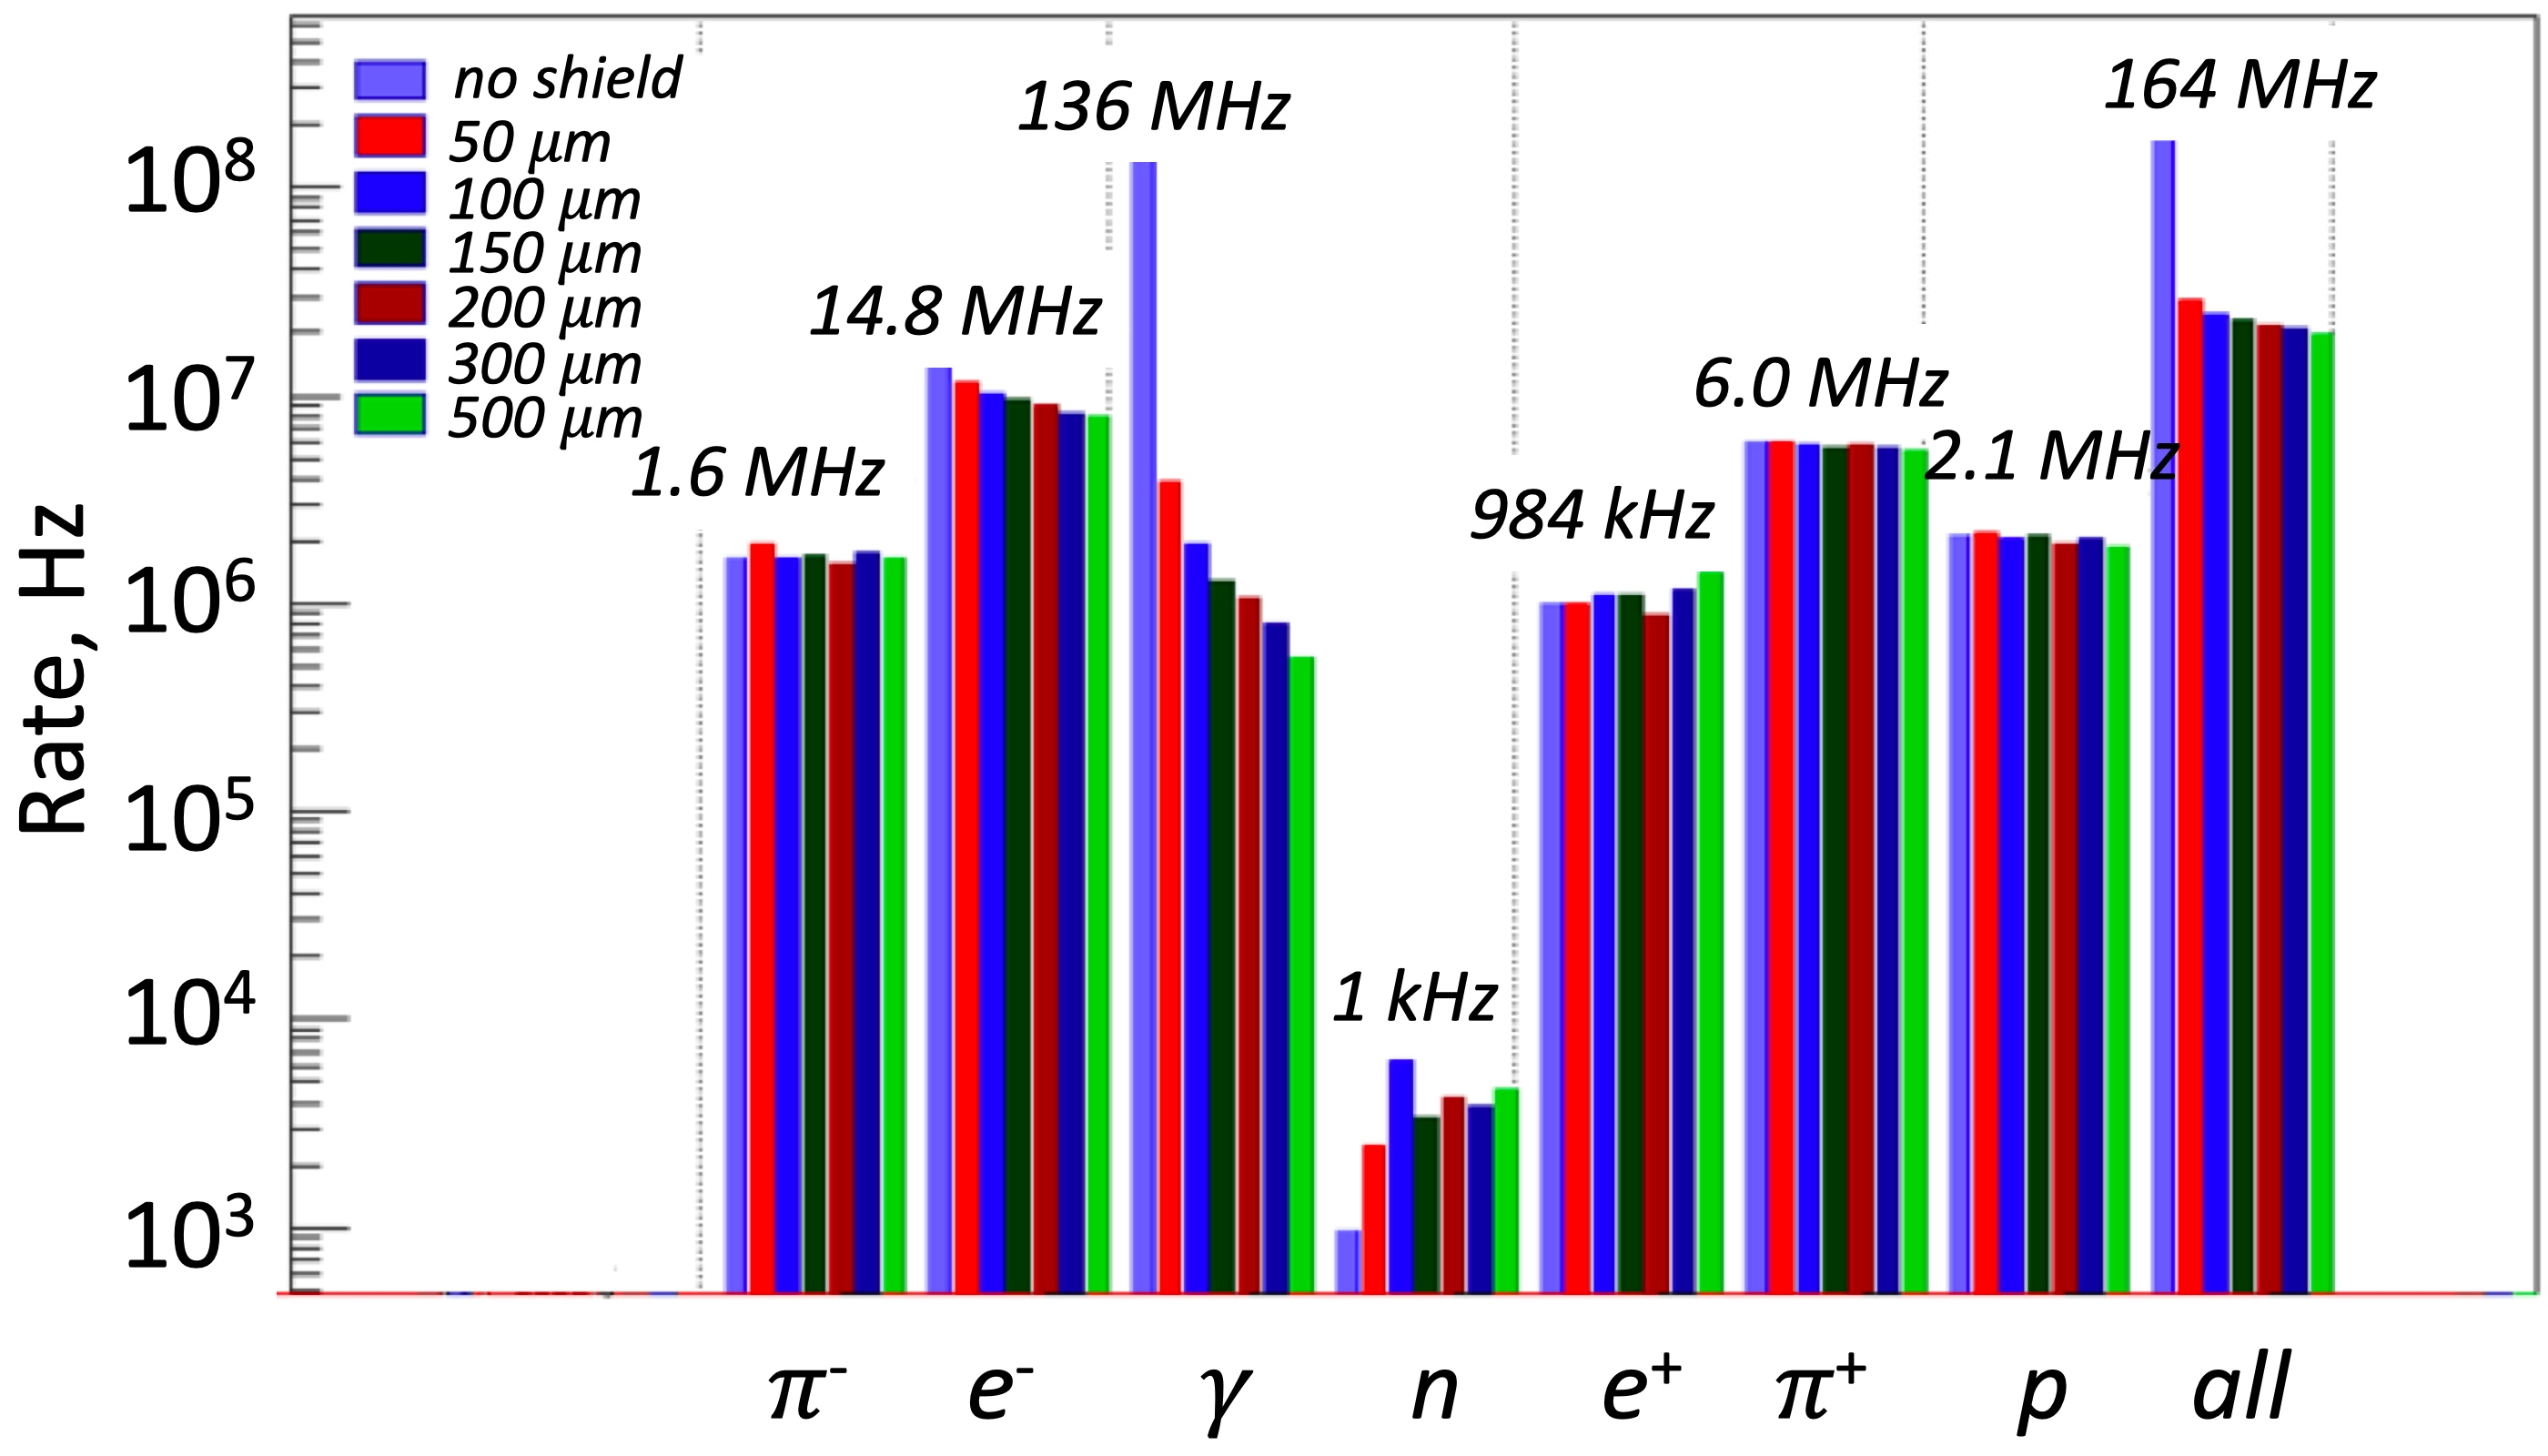
\includegraphics[width=1.0\columnwidth,keepaspectratio]{rates-l1.jpg}
\caption{Rates in the first SVT layer for different tungsten shield thickness from 50 to 500 $\mu$m for a liquid hydrogen target at the nominal CLAS12 operating luminosity. No energy threshold cut applied.}
\label{fig:rates-l1}
\end{figure}

\subsection{Magnetic Field}

Due to the constrains on the maximum length of the cables, the readout, slow controls, and power supply crates are installed on a movable service cart within few meters from the detector. To assess the potential impact of the solenoid field on the SVT DAQ, a magnetic field map was simulated for the location of the power supply and readout crates. Fig.~\ref{fig:solenoid-field}) shows that the maximum strength of the field for the crates is at an acceptable level of 100 G.

\begin{figure}[hbt] 
\centering 
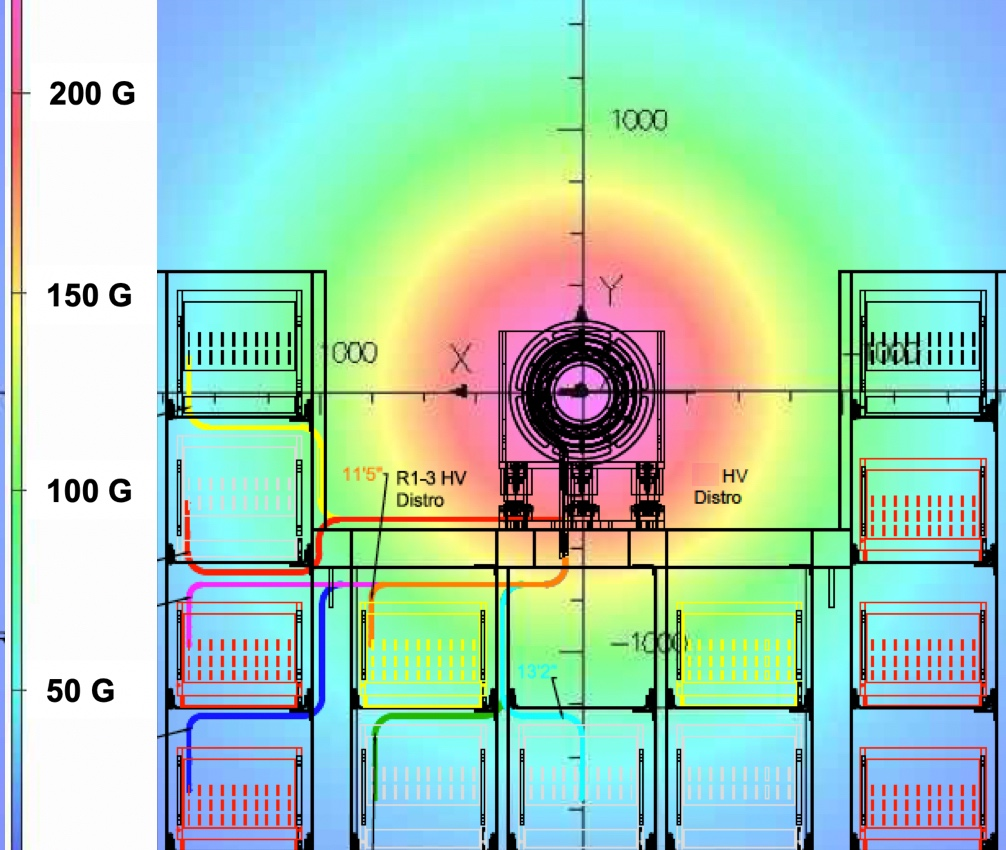
\includegraphics[width=1.0\columnwidth,keepaspectratio]{solenoid-field.jpg}
\caption{Solenoid field map at the location of the SVT service cart.}
\label{fig:solenoid-field}
\end{figure}

%\subsection{Occupancies}

%\subsection{Alignment}

%Validation of alignment procedures was performed on Monte Carlo simulation and cosmic data. Detector alignment procedure is using a least squares approach of a Millepede II algorithm \cite{Millepede}. The dependence of the residuals on the track parameters is explicitly taken into account. The alignment code uses the partial derivatives of the distance of closest approach (DOCA) taken with respect to the track parameters and the SVT geometry. This approach accounts for correlated shifts among the geometry parameters. Results of alignment correction for one of the SVT modules are shown in Fig.~\ref{fig:alignment}. Only shifts in the sensor plane were taken into account in the alignment procedure for this plot.

%\begin{wrapfigure}{l}{0.5\columnwidth}
%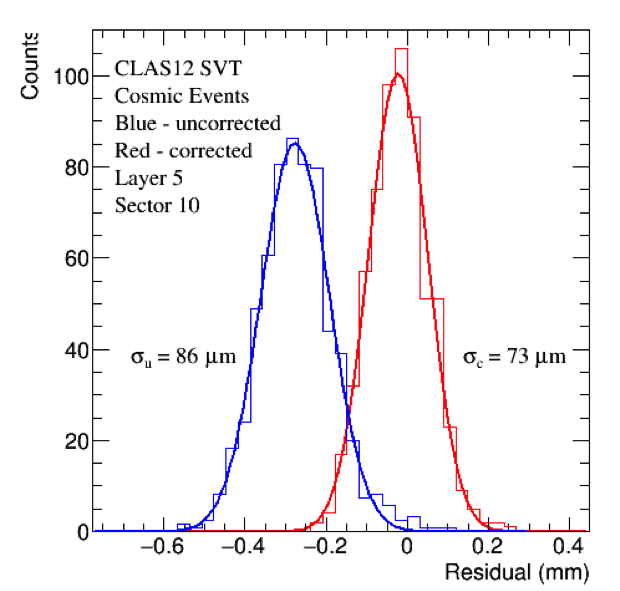
\includegraphics[width=1.0\columnwidth]{alignment.png}
%\caption{Alignment of the SVT module.}
%\label{fig:alignment}
%\end{wrapfigure}

%\subsection{Resolutions}


%\subsection{Efficiencies}

